\section{Conditional consistency of output-space fusion}
\label{app:fusion_consistency}
Let $\bm u_\alpha=\alpha\bm u_1+\beta\bm u_2$ and $p_\alpha=\alpha p_1+\beta p_2$, where $\beta=1-\alpha$, $\alpha\in[0,1]$ is constant in space and time over the window, and both candidates share a mesh, parameter, time grid, and pressure gauge. For a common linear operator $D_h$, $D_h\bm u_\alpha=\alpha D_h\bm u_1+\beta D_h\bm u_2$. Thus zero discrete divergence, a zero-mean pressure gauge, and identical affine boundary constraints are preserved only to the extent that both candidates satisfy them.

\paragraph{Nonlinear residuals.}
For a fixed bilinear discretization $N_h$, set $\delta\bm u=\bm u_1-\bm u_2$. Bilinearity gives
\begin{equation}
N_h(\bm u_\alpha,\bm u_\alpha)
=\alpha N_h(\bm u_1,\bm u_1)+\beta N_h(\bm u_2,\bm u_2)
-\alpha\beta N_h(\delta\bm u,\delta\bm u).
\end{equation}
With the sign convention
$R_u(\bm u,p)=\partial_t\bm u-\bm f_h-L_h\bm u+N_h(\bm u,\bm u)+G_hp$, one obtains
\begin{equation}
R_u(\bm u_\alpha,p_\alpha)
=\alpha R_u(\bm u_1,p_1)+\beta R_u(\bm u_2,p_2)
-\alpha\beta N_h(\delta\bm u,\delta\bm u).
\end{equation}
For the pressure residual
$R_p(\bm u,p)=A_hp-[\bm s_0+S_1\bm u+B_p(\bm u,\bm u)]$, with fixed bilinear $B_p$, similarly
\begin{equation}
R_p(\bm u_\alpha,p_\alpha)
=\alpha R_p(\bm u_1,p_1)+\beta R_p(\bm u_2,p_2)
+\alpha\beta B_p(\delta\bm u,\delta\bm u).
\end{equation}
These identities distinguish the candidates' existing residuals from the additional fusion defect. They are conditional algebraic identities, not measurements of the CFD residual: state-dependent limiters or other non-bilinear discretizations require their actual discrete operators.

\paragraph{Energy and phase cancellation.}
For $E(\bm u)=\tfrac12\|\bm u\|_M^2$ with a common positive quadrature matrix,
\begin{equation}
E(\bm u_\alpha)=\alpha E(\bm u_1)+\beta E(\bm u_2)
-\frac{\alpha\beta}{2}\|\bm u_1-\bm u_2\|_M^2.
\end{equation}
Candidate disagreement can therefore reduce the blend's energy relative to the weighted candidate energies, including through phase cancellation. This does not imply that its energy is below the reference solution or below both candidates. Since the blend is not fed back into either specialist, this term is not a recurrent dissipative modification of their reduced dynamics. Empirical residual and phase-sensitive evaluations remain separate from these identities.

\subsection{Measured common-grid diagnostics}
\label{app:fusion_measured}
We evaluate both candidates, their frozen T2-C blend, and the common
POD-reconstructed reference on all 16 held-out windows at each square-cylinder
interface ($K=24$, output spacing 4). No window is selected by prediction
quality. These are reconstructed-field diagnostics, not residuals of the
original OpenFOAM finite-volume equations and not errors against unprojected
CFD fields.

\paragraph{Operators and averaging.}
On the common 9,400-cell grid, quadratic local least-squares fits define
$D_x,D_y$ and $L$. The initial stencil has 24 nearest cells, with independent
coordinate scaling; it is expanded only if the polynomial matrix is
rank-deficient or has condition number above $10^6$. A 36-neighbor version
checks sensitivity. Actual stencils contain at most 72 cells. Both versions
differentiate a manufactured quadratic polynomial with maximum absolute
error below $1.4\times10^{-10}$. We use
\begin{equation}
\widehat R_u=\delta_t\bm u+N_D(\bm u,\bm u)+\nabla_Dp-Re^{-1}L\bm u,
\qquad
\widehat R_p=Lp+D_xN_{D,x}+D_yN_{D,y},
\end{equation}
where $N_D(\bm u,\bm u)=uD_x\bm u+vD_y\bm u$.
Residual norms use area-weighted RMS over the interior wake
$6\leq x\leq16$, $1\leq y\leq3$ (2,627 cells).
Centered time differences and summary statistics use output steps 2--23.
The nonzero reference residual includes POD truncation and spatial/temporal
differentiation error; it is not a solver convergence tolerance. Windows
are averaged within each parameter, then parameters equally. The two
parameters per interface each contribute eight overlapping windows;
these windows are not independent experimental replications.

\begin{table}[H]
\centering\small
\caption{Measured square-interface diagnostics with the 24-neighbor initial
stencil. Energy error is $|E-E_{\rm ref}|/E_{\rm ref}$ in percent over the
whole domain; residuals are interior RMS. All columns average steps 2--23.
Reference denotes POD-reconstructed CFD, not raw CFD.}
\label{tab:fusion_residual_measured}
\begin{tabular}{@{}llrrr@{}}
\toprule
Interface & Field & Energy error (\%) & $\|\widehat R_u\|$ & $\|\widehat R_p\|$\\
\midrule
S--H & Reference & 0 & 0.00460 & 0.03395\\
& Steady & 2.81100 & 0.00530 & 0.03674\\
& Hopf & 0.14296 & 0.00607 & 0.03513\\
& T2-C & 0.17641 & 0.00520 & 0.03421\\
\midrule
H--P & Reference & 0 & 0.11486 & 0.03736\\
& Periodic & 0.09163 & 0.11627 & 0.03785\\
& Hopf & 0.17298 & 0.11189 & 0.04047\\
& T2-C & 0.05974 & 0.11408 & 0.03631\\
\bottomrule
\end{tabular}
\end{table}

\paragraph{Identities versus measured accuracy.}
The maximum absolute discrepancies in the energy, momentum-residual and
pressure-residual identities are $1.2\times10^{-15}$,
$7.4\times10^{-15}$ and $6.1\times10^{-14}$, respectively, across both
stencils and all windows. These values verify the implementation of the
identities, not physical accuracy. The mean blend-energy deficit relative
to reference energy is $0.00314\%$ (S--H) and $0.00181\%$ (H--P), distinct
from the energy-error column in Table~\ref{tab:fusion_residual_measured}.
T2-C has a lower measured pressure residual than either candidate for both
interfaces and both stencils. However, it does not minimize every diagnostic:
the Hopf candidate has a smaller H--P momentum residual and a smaller S--H
energy error. Changing the stencil also changes residual magnitudes
substantially. Thus output blending is not a general residual minimizer,
nor do these results establish discrete conservation or stability.

\paragraph{Phase diagnostics.}
A transverse-velocity probe is fixed geometrically at the cell nearest
$(8,2.5)$. We detrend each signal and compare Hilbert phases with the
reference. A window is marked unresolved if the reference dominant
non-Nyquist Fourier component spans fewer than two cycles or its detrended
standard deviation is below $10^{-5}$. None of the 16 S--H windows and only
15 of the 16 H--P windows pass this screening. Even passing this necessary
screen is not evidence that temporal aliasing or Hilbert endpoint effects
are absent. We therefore report phase traces as short-window diagnostics,
not as evidence for a general reduction of phase error or long-time
phase stability.

\begin{figure}[H]
\centering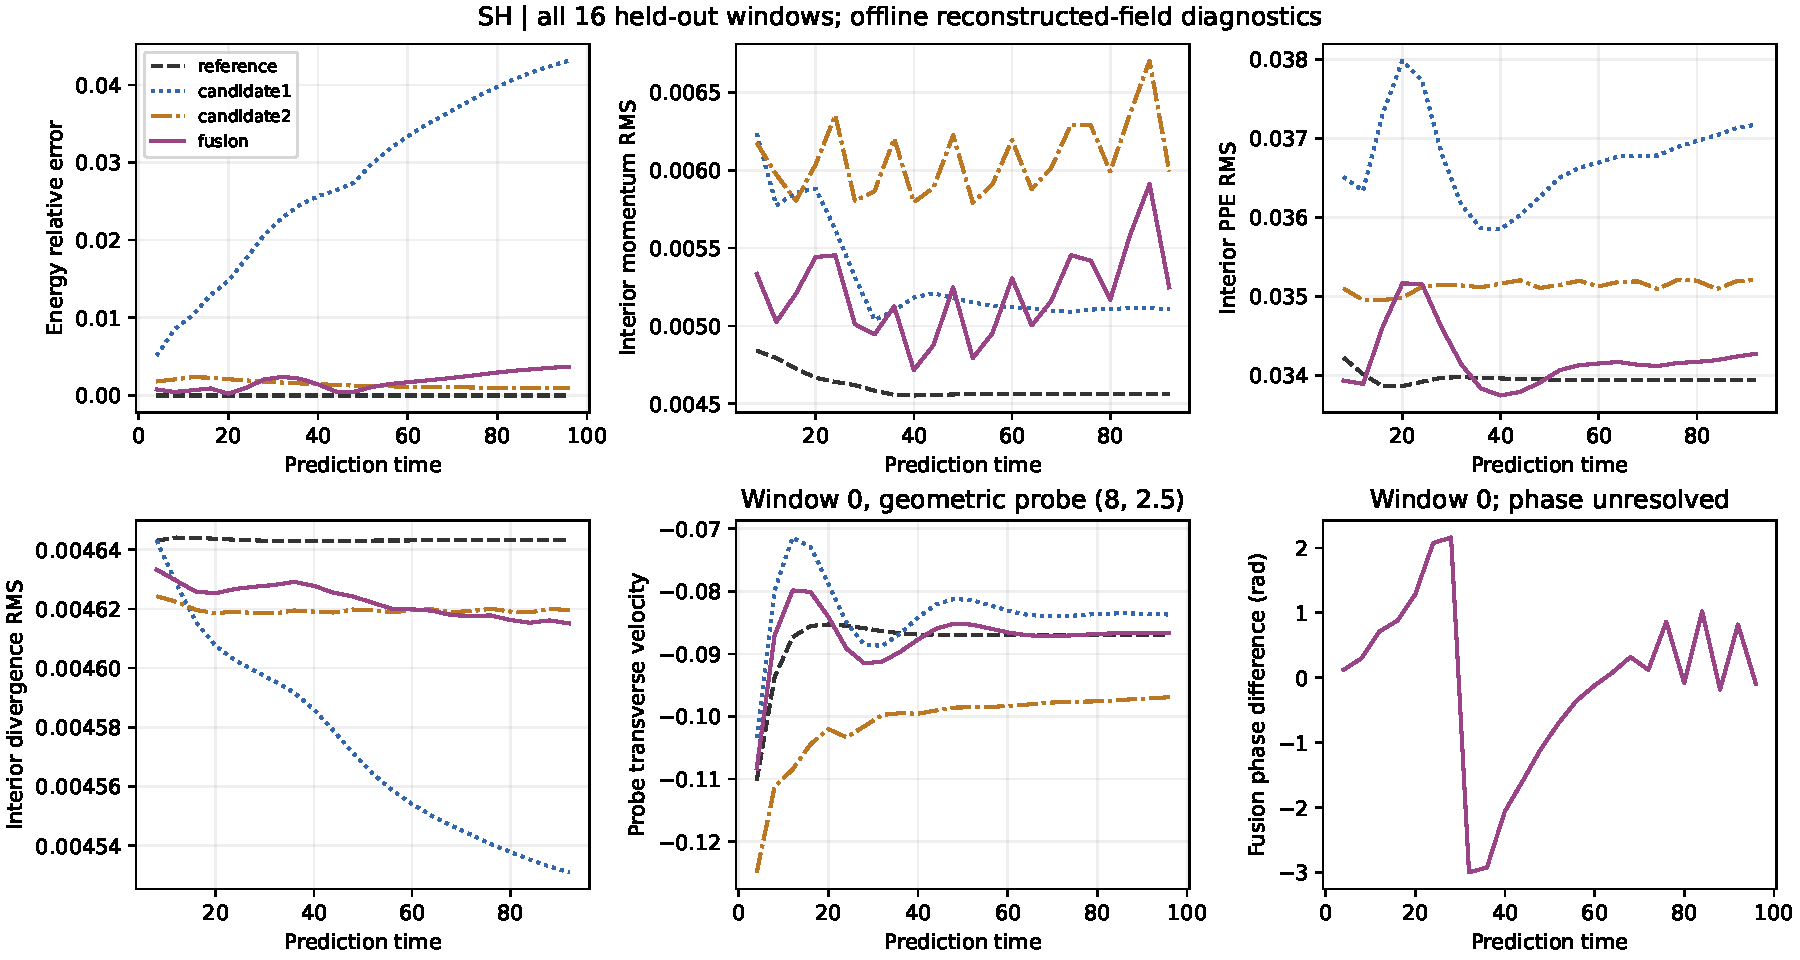
\includegraphics[width=\linewidth]{figures/round3_sh_diagnostics.pdf}
\caption{S--H diagnostics: the first four panels average all 16 windows;
the last two show the first frozen window, not a best-case selection.
Candidate 1 is Steady and candidate 2 is Hopf. Reference is POD-reconstructed
CFD. The unresolved phase trace is descriptive only.}
\end{figure}
\begin{figure}[H]
\centering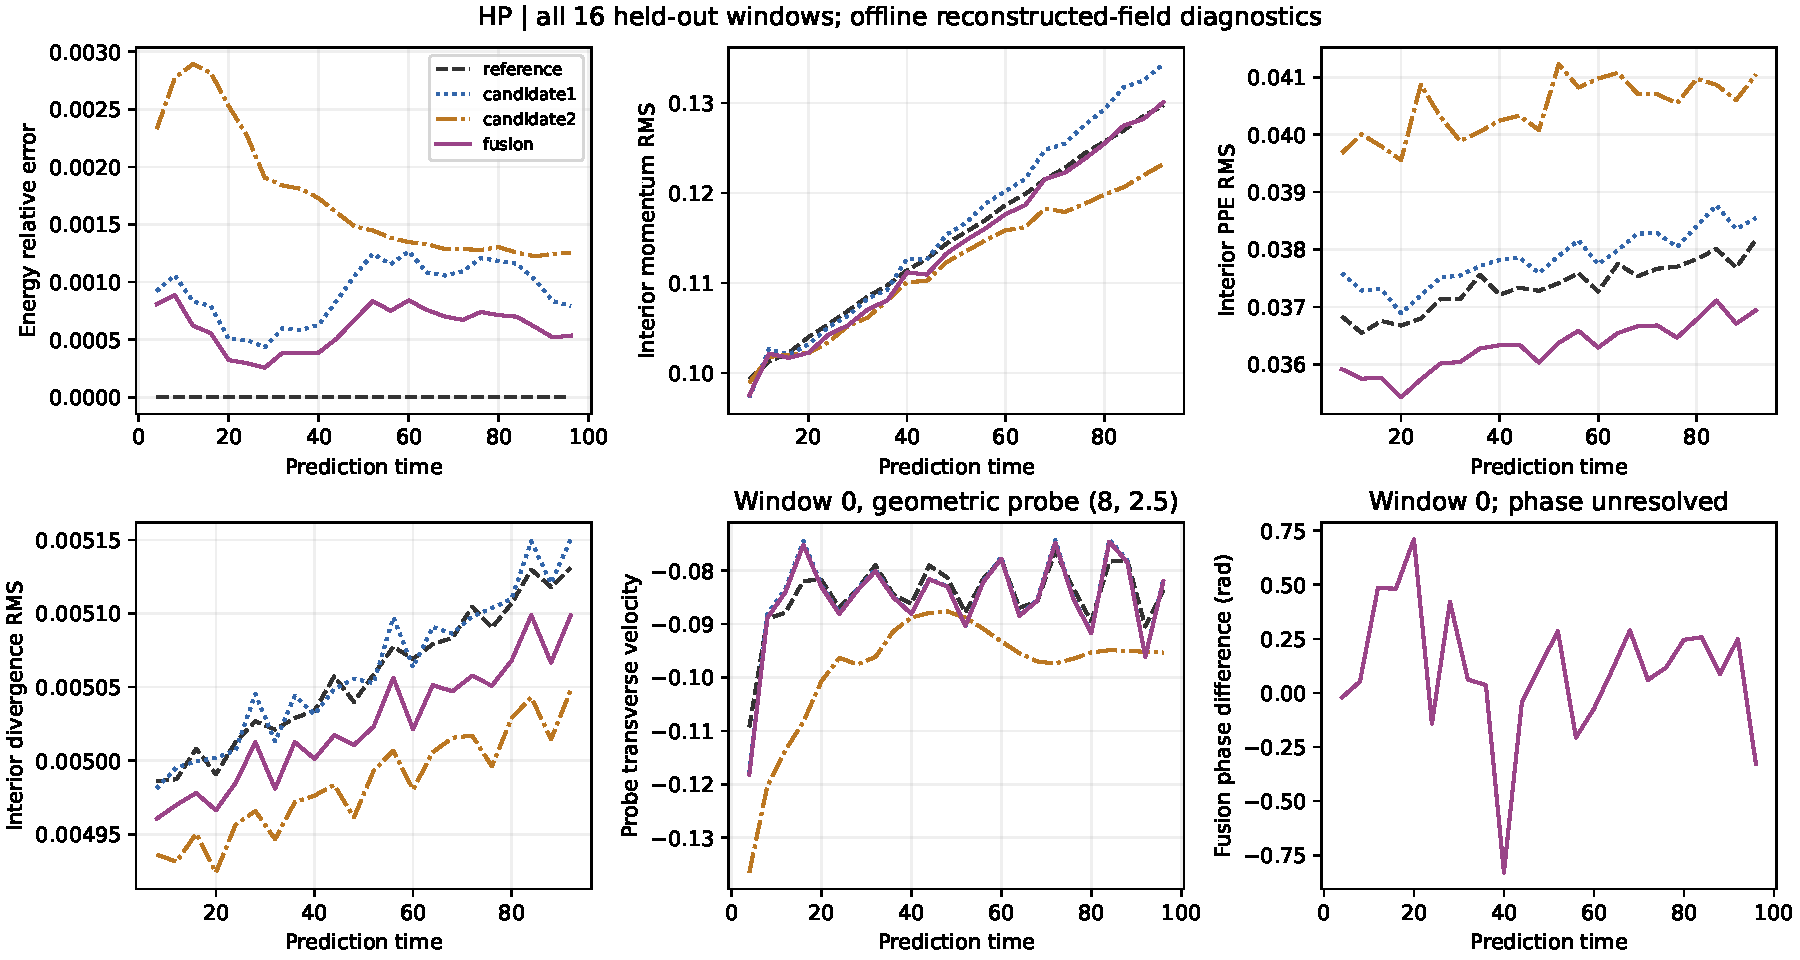
\includegraphics[width=\linewidth]{figures/round3_hp_diagnostics.pdf}
\caption{H--P diagnostics under the same protocol. Candidate 1 is Periodic
and candidate 2 is Hopf. The first four panels average all 16 windows;
the probe and phase panels show the first frozen window, which is
unresolved by the stated phase screen.}
\end{figure}
\begin{figure}[H]
\centering
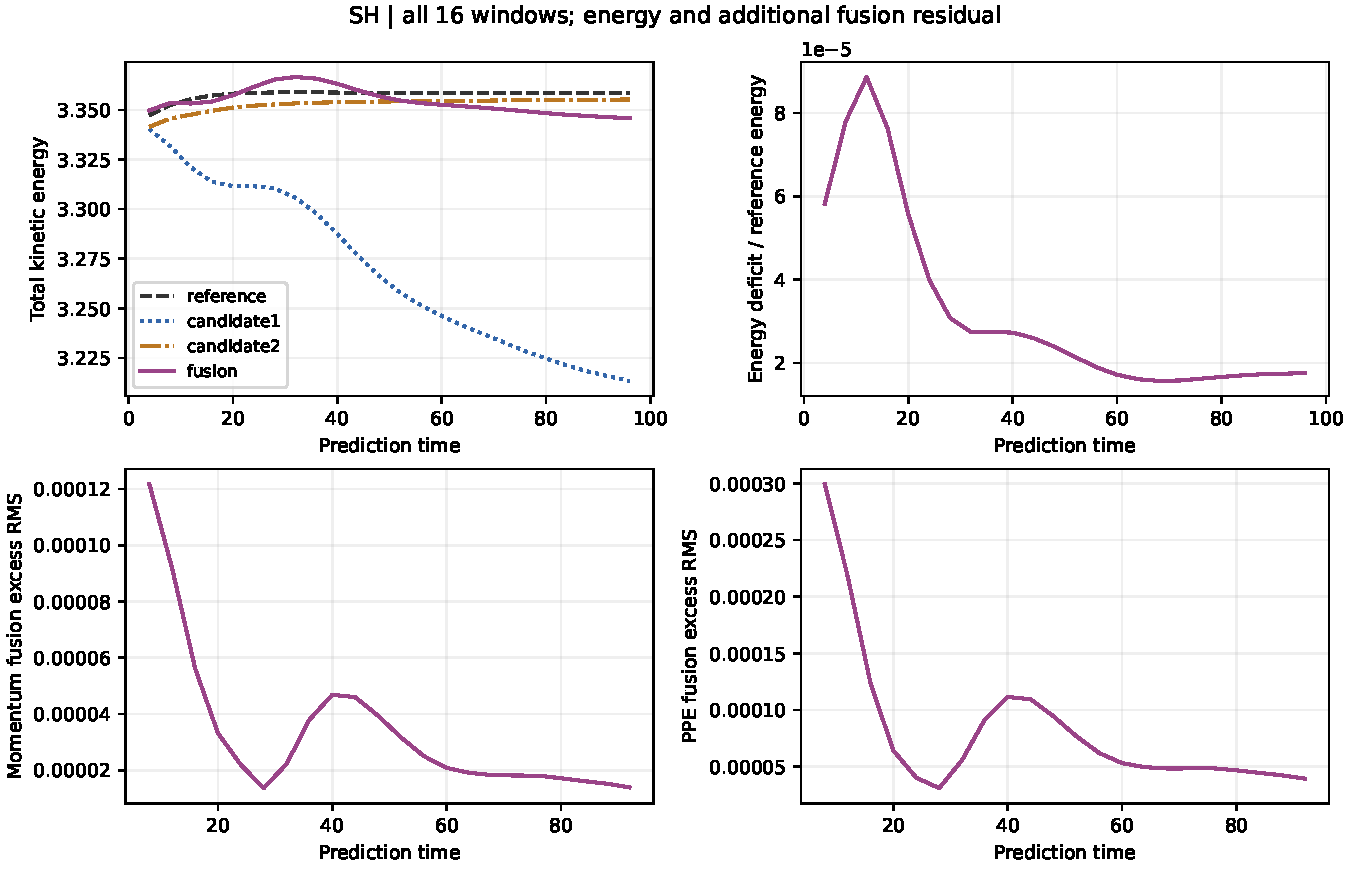
\includegraphics[width=.95\linewidth]{figures/round3_sh_energy_excess.pdf}
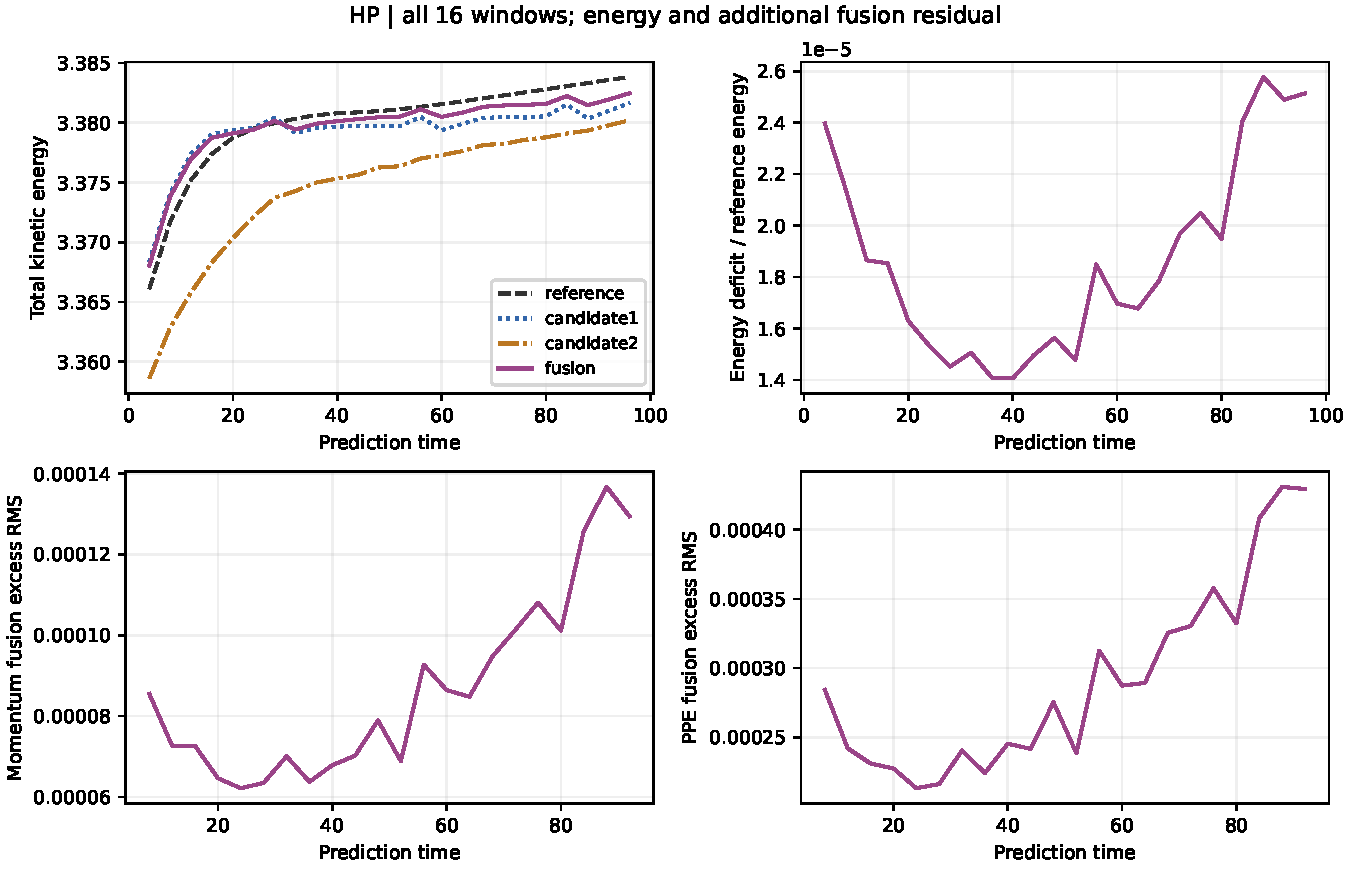
\includegraphics[width=.95\linewidth]{figures/round3_hp_energy_excess.pdf}
\caption{Actual kinetic energy and additional fusion defects averaged over
all windows. The energy deficit is measured relative to the weighted
candidate energies, normalized by reference energy; it is not the energy
error. Momentum and pressure excesses are differences from the
weighted candidate residuals, not the total fused residuals.}
\end{figure}
